3\subsection{Kraftfelder}
\label{mdforcefields}

Zentrales Element molekulardynamischer Methoden sind Kraftfelder $\vec F(X)$, auch Potentiale $V(X)$ genannt, welche die Interaktionen der simulierten Teilchen beschreiben.
Für verschiedene Materialien existieren spezielle Potentialformulierungen, die für unterschiedliche Elemente wiederum eigene Potentialparametrisierungen in Form von Potentialdateien zur Verfügung stellen.
Im Folgenden soll eine Auswahl dieser Potentialformulierungen kurz in ihrer Funktionsweise vorgestellt werden.

\subsubsection{Paar-Potentiale}

Das einfachste MD-Potential ist das Paarpotential, welches eine Interaktion zwischen jeweils zwei benachbarten Atomen modelliert, wodurch sich das System auf Gleichungen~\ref{eq:pairforce} und~\ref{eq:pairenergy} reduziert.
Stellvertretend steht das Lennard-Jones-Potential zur Darstellung von allgemeinen Fluiden (Gleichung~\ref{eq:lennardjones}) oder das damit verwandte Bucking\-ham-Potential (Abbildung~\ref{fig:mdpairpotentials}).
Allen Paar-Potentialen ist gemein, eine rein radiale Abhängigkeit $V(r_ij)$ zu besitzen, die oftmals einen charakteristischen Bindungsabstand in Abhängigkeit der Parameter bildet, welcher sich als Minimum in den Potentialen äußert.
Unterhalb dieses Radius' dominiert ein repulsiver Term, wo hingegen oberhalb davon ein leicht attraktiver Term vorherrscht, der sich für große Radien einem konstanten Wert annähert und deshalb mit einem Cutoff-Radius $r_\text{cut}$ versehen ist.

\begin{equation}
  \label{eq:pairforce}
  \vec F_{ij}(r_{ij}) = \vec\nabla V(r_{ij})
\end{equation}
\begin{equation}
  \label{eq:pairenergy}
  E = \sum_i\sum_{j \neq i}{V(r_{ij})}
\end{equation}
\begin{equation}
  \label{eq:lennardjones}
  V_\text{LJ}(r_{ij}) = 4 \epsilon \left[\left(\frac{\sigma}{r_{ij}}\right)^{12} - \left(\frac{\sigma}{r_{ij}}\right)^{6}\right]
\end{equation}

\begin{figure}
  \centering
  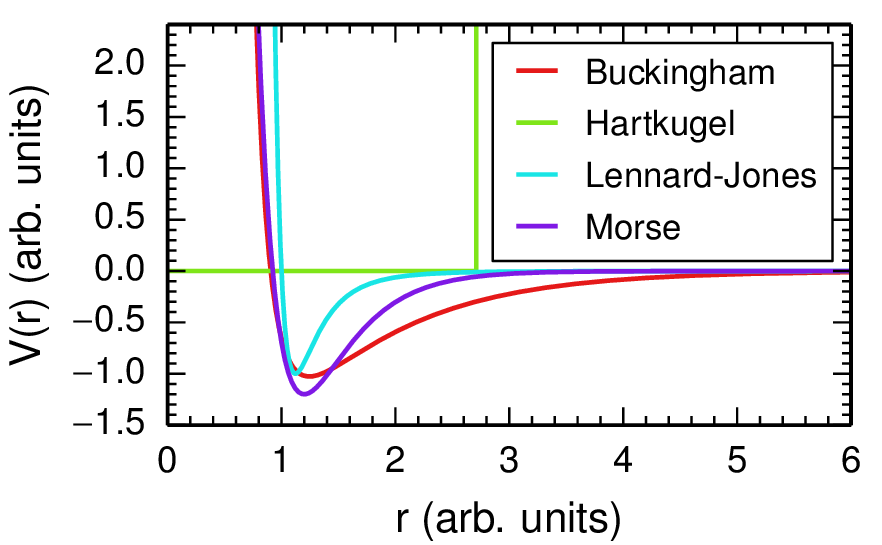
\includegraphics[width=0.5\textwidth]{mdpotplot}
  \caption{Beispiele einfacher Paarpotentiale}
  \label{fig:mdpairpotentials}
\end{figure}

Zwar zeigen Paarpotentiale gute thermodynamische Eigenschaften bei hoher Effizienz, doch können sie aufgrund ihrer Schlichtheit kein atomistischen Strukturen verlässlich vorhersagen, weshalb die umfangreicheren Mehrteilchen-Potentiale entwickelt wurden.

\subsubsection{N-Teilchen-Potentiale}

N-Teilchen-Potentiale erweitern Paarpotentiale um weitere Terme, die von einer festen Anzahl an Teilchen abhängen, beispielsweise Winkel- und Torsionsabhängigkeiten.

\begin{equation}
  \label{eq:nbody-energy}
  E = \sum_i\sum_{j \neq i}{V_2\left(r_{ij}\right)} + \sum_i\sum_{j \neq i}\sum_{i \neq k \neq j}{V_3\left(r_{ij}, r_{ik}, \theta_{ijk}\right)} + \dots
\end{equation}
\todo{letzte Summe: Indizes aufspalten}

Obwohl sich mit N-Teilchen-Potentialen komplexere Systeme betrachten lassen, zeigen sie die gleichen Schwachstellen wie Paarpotentiale, benötigen aber eine größere Anzahl an Parametern,
Zwar gibt es erfolgreiche \todo{kommerzielle} Anwendungen für Biomoleküle (\todo{CHARMM} \todo{GROMACS} \todo{AMBER}), die allerdings aufgrund ihrer Spezialisierung nicht auf andere Stoffsysteme wie Festkörper oder Oberflächen übertragbar sind.

\subsubsection{Embedded Atom Model}

Das Embedded Atom Model (EAM) besteht aus einem Paarpotential $V_{\alpha\beta}(r_{ij})$ für jedes Atom $i$ sowie einer Einbettungsfunktion $F_\alpha$, welche die Energie des Atomes in Abhängigkeit der angenäherten lokalen Elektronendichte $\rho_\beta(r_{ij})$ modelliert (Gleichung~\ref{eq:eam-energy}).\todo{Referenz}
So lassen sich metallische Bulks und Oberflächen simulieren, für die $\alpha$ und $\beta$ verschiedene Spezies darstellen, doch führt die Formulierung für andere Systeme zwangsläufig zur Bildung von Clustern\todo{warum?}.
Für eine Vielzahl an Metallen und Legierungen findet man in \todo{wie beispielsweise ASD}Potentialdatenbanken fertige Parametrisierungen\todo{Referenz auf Datenbank und passende Paper}, von denen viele zusätzlich zu den strukturellen Eigenschaften auch thermodynamisches Verhalten recht gut modellieren (Abschnitt~\ref{goldthermo}).

\begin{equation}
  \label{eq:eam-energy}
  E = \sum_i\left[F_\alpha\left(\sum_{j\neq i}{\rho_\beta\left(r_{ij}\right)}\right) + \frac{1}{2}\sum_{j\neq i}{V_{\alpha\beta}\left(r_{ij}\right)}\right]
\end{equation}

\subsubsection{Modified Embedded Atom Model}

Als Erweiterung des EAM-Potentials wurden MEAM-Potentiale entwickelt, die neben Metallen und Legierungen auch Metalloxide und andere Mischsysteme ermöglichen sollen. \todo{Referenz auf Baskes}
Sie basieren auf der gleichen Funktionsweise, stellen die Einbettungsenergie aber in Abhängigkeit einer umfangreicheren Formulierung der lokalen Elektronendichte dar.
An dieser Stelle soll neben der oberflächlichen Formel in Gleichung~\ref{eq:meam-energy} auf die ursprüngliche Publikation von Baskes \todo[inline]{Ref!} verwiesen werden.

\begin{equation}
  \label{eq:meam-energy}
  E = \sum_i\left[F_\alpha\left(\bar{\rho_i}\right) + \frac{1}{2}\sum_{j\neq i}{V_{ij}\left(r_{ij}\right)}\right]
\end{equation}

\subsubsection{Reactive Force Fields}

Reaktive Kraftfelder (Reactive Force Fields, ReaxFF) wurden \todo{Jahreszahl und Ref auf van Duin}mit dem Ziel entwickelt, Reaktionen zwischen Molekülen mit molekulardynamischen Methoden beschreiben zu können.
Mangels expliziter Beschreibung der involvierten Elektronen war die Beschreibung von Bindungen zuvor nur mit \todo{DFT?}Elektronenstrukturrechnungen möglich, denen eine obere Grenze von wenigen hundert Atomen gesetzt ist, \todo{Nebensatz sinnlos}und selbst dann die Berechnung dynamischer Eigenschaften mit einem immensen Rechenaufwand verbunden ist.
Durch Beschreibung der Über- und Unterkoordination der Atome innerhalb ihrer Nachbarschaft, zusätzlich zum Ladungsaustausch zwischen den Atomen, Van-der-Waals- und elektrostatischen Kräften, lassen sich mit der ReaxFF-Formulierung Bindungen während der Simulation dynamisch formen und lösen, wodurch Reaktionen ermöglicht werden.
Gleichung~\ref{eq:reaxformulation} und Tabelle~\ref{tab:reaxenergies} geben einen kurzen Überblick über die Bestandteile der Gesamtenergie, von denen die meisten Terme über die Bindungsordnung berechnet werden, welche sich aus Beiträgen für $\sigma$-, $\pi$- und Doppel-$\pi$-Bindungen aus dem Bindungsabstand zusammen setzt.
Darüber hinaus werden einige Terme durch Taper-Korrektur\todo{ref} in der Nähe des Cutoff-Abstands auf 0 gesenkt, um Diskontinuitäten zu vermeiden und einen fließenden Übergang zwischen Bindungszuständen zu ermöglichen.

\begin{align}
  \label{eq:reaxformulation}
  E_\text{system} =~& E_\text{bond} + E_\text{lp} + E_\text{over} + E_\text{under} + E_\text{val} + E_\text{pen} + E_\text{coa} + E_\text{C2} \\
  \nonumber  & + E_\text{tors} + E_\text{conj} + E_\text{H-bond} + E_\text{vdWaals} + E_\text{Coulomb}
\end{align}

\todo{Referenz auf Equations\_Reax.pdf}

\begin{table}
  \caption[ReaxFF Energiebeiträge]{ReaxFF Energiebeiträge aus Gleichung~\ref{eq:reaxformulation}}
  \label{tab:reaxenergies}
  \begin{tabularx}{\textwidth}{|llX|}
    \hline
    \textbf{Term}      & \textbf{Beitrag}            & \textbf{Kommentar}                            \\
    \hline
    $E_\text{bond}$    & Bindungsenergien            & Berechnung über Bindungsordnung               \\
    $E_\text{lp}$      & freie Elektronenpaare       & über Bindungsordnungssumme am Atomzentrum     \\
    $E_\text{over}$    & Überkoordinationen          & unter Ausschluss freier Elektronenpaare       \\
    $E_\text{under}$   & Unterkoordinationen         & nur bei unterkoordinierten $\pi$-Bindungen    \\
    $E_\text{val}$     & Bindungswinkel              & Optimum abhängig von Elektronenkonfiguration  \\
    $E_\text{pen}$     & Strafenergien               & Fehlerkorrektur bei Winkeln mit Doppelbindung \\
    $E_\text{coa}$     & Drei-Teilchen-Konjugationen & Stabilisierung von NO$_2$-Gruppen             \\
    $E_\text{C2}$      & Dreifachbindungskorrektur   & Stabilisierung der Dreifachbindung von C$_2$  \\
    $E_\text{tors}$    & Torsionsbarrieren           &                                               \\
    $E_\text{conj}$    & Vier-Teilchen-Konjugationen & Konjugation bei Kohlenwasserstoffen           \\
    $E_\text{H-bond}$  & Wasserstoffbrücken          &                                               \\
    $E_\text{vdWaals}$ & Van-der-Waals-Kräfte        &                                               \\
    $E_\text{Coulomb}$ & Coulomb-Kräfte              &                                               \\
    \hline
  \end{tabularx}
\end{table}

Aus den Termen des ReaxFF-Potentials geht hervor, dass es ursprünglich für Reaktionen von organischen Molekülen entwickelt wurde, doch es hat sich als vielseitig genug herausgestellt, auch eine Vielzahl anderer Materialien wie Kristalle und nichtorganische Verbindungen simulieren zu können.
Die einzige Abhängigkeit besteht zum Trainingssatz, also den Test-Strukturen, an deren Werte die Parametrisierung des Reax-Kraftfeldes angepasst wurde.
So kann die Parametrisierung am Ende maximal die Strukturen und Materialien zuverlässig unterstützen, für die sie ursprünglich erstellt wurde.

In den letzten fünf Jahren haben Reactive Force Fields jedoch langsam an Aufmerksamkeit gewonnen, so dass die Zahl spezialisierter Parametrisierungen stetig zunimmt.
Es gibt auch Bestrebungen, sich ergänzende ReaxFF-Parametrisierungen zu kombinieren und somit mit einer Parametrisierung jedes gewünschte System betrachten zu können.
Besonders in kommerzieller MD-Software\todo{Referenz auf GULP} versucht man so, dem Nutzer ein umfassendes Paket für die Simulation beliebiger Strukturen zu präsentieren, ohne ihm aber die Grenzen des Parametersatzes erkenntlich zu machen.
